% This file was created with tikzplotlib v0.10.1.
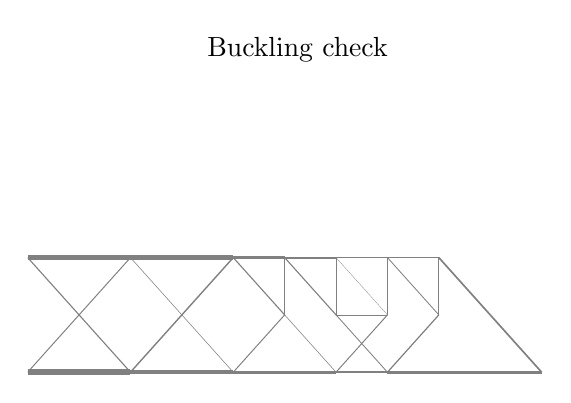
\begin{tikzpicture}

\definecolor{darkgray176}{RGB}{176,176,176}
\definecolor{gray}{RGB}{128,128,128}

\begin{axis}[
hide x axis,
hide y axis,
tick align=outside,
tick pos=left,
title={Buckling check},
x grid style={darkgray176},
xmin=0, xmax=10.5,
xtick style={color=black},
y grid style={darkgray176},
ymin=-2.86209677419355, ymax=4.96209677419355,
ytick style={color=black}
]
\path [draw=gray, line width=1.99999999999875pt]
(axis cs:0,0)
--(axis cs:1,0);

\path [draw=gray, line width=0.358089753489192pt]
(axis cs:0,0)
--(axis cs:1,1);

\path [draw=gray, line width=2pt]
(axis cs:1,0)
--(axis cs:2,0);

\path [draw=gray, line width=1.4285714285343pt]
(axis cs:2,0)
--(axis cs:3,0);

\path [draw=gray, line width=0.404061017836389pt]
(axis cs:2,0)
--(axis cs:1,1);

\path [draw=gray, line width=0.506415385985737pt]
(axis cs:2,0)
--(axis cs:3,1);

\path [draw=gray, line width=1.42857142853598pt]
(axis cs:3,0)
--(axis cs:4,0);

\path [draw=gray, line width=1.20446556028245pt]
(axis cs:4,0)
--(axis cs:5,0);

\path [draw=gray, line width=0.202030508872148pt]
(axis cs:4,0)
--(axis cs:3,1);

\path [draw=gray, line width=0.35808975350254pt]
(axis cs:4,0)
--(axis cs:5,1);

\path [draw=gray, line width=1.20446556028132pt]
(axis cs:5,0)
--(axis cs:6,0);

\path [draw=gray, line width=0.358089753518642pt]
(axis cs:6,0)
--(axis cs:7,1);

\path [draw=gray, line width=0.857142857127464pt]
(axis cs:6,0)
--(axis cs:7,0);

\path [draw=gray, line width=0.202030508912975pt]
(axis cs:6,0)
--(axis cs:5,1);

\path [draw=gray, line width=0.303045763355493pt]
(axis cs:7,0)
--(axis cs:6,1);

\path [draw=gray, line width=0.438568589113824pt]
(axis cs:7,0)
--(axis cs:8,1);

\path [draw=gray, line width=1.10637226328383pt]
(axis cs:7,0)
--(axis cs:8,0);

\path [draw=gray, line width=1.10637226328162pt]
(axis cs:8,0)
--(axis cs:9,0);

\path [draw=gray, line width=1.10637226328196pt]
(axis cs:9,0)
--(axis cs:10,0);

\path [draw=gray, line width=0.606091526713084pt]
(axis cs:10,0)
--(axis cs:9,1);

\path [draw=gray, line width=0.404061017837327pt]
(axis cs:1,1)
--(axis cs:0,2);

\path [draw=gray, line width=0.358089753486455pt]
(axis cs:1,1)
--(axis cs:2,2);

\path [draw=gray, line width=0.202030508870817pt]
(axis cs:3,1)
--(axis cs:2,2);

\path [draw=gray, line width=0.506415385982235pt]
(axis cs:3,1)
--(axis cs:4,2);

\path [draw=gray, line width=0.404061017821728pt]
(axis cs:5,1)
--(axis cs:4,2);

\path [draw=gray, line width=0.301116390064781pt]
(axis cs:5,1)
--(axis cs:5,2);

\path [draw=gray, line width=0.0714285714300622pt]
(axis cs:6,1)
--(axis cs:7,1);

\path [draw=gray, line width=0.404061017803535pt]
(axis cs:6,1)
--(axis cs:5,2);

\path [draw=gray, line width=0.150558195028537pt]
(axis cs:6,1)
--(axis cs:6,2);

\path [draw=gray, line width=0.101015254447398pt]
(axis cs:7,1)
--(axis cs:6,2);

\path [draw=gray, line width=0.26077444329327pt]
(axis cs:7,1)
--(axis cs:7,2);

\path [draw=gray, line width=0.303045763357521pt]
(axis cs:8,1)
--(axis cs:7,2);

\path [draw=gray, line width=0.428571428558497pt]
(axis cs:8,1)
--(axis cs:8,2);

\path [draw=gray, line width=0.606091526715564pt]
(axis cs:9,1)
--(axis cs:8,2);

\path [draw=gray, line width=1.85714285710452pt]
(axis cs:0,2)
--(axis cs:1,2);

\path [draw=gray, line width=1.85714285710567pt]
(axis cs:1,2)
--(axis cs:2,2);

\path [draw=gray, line width=1.5714285714332pt]
(axis cs:2,2)
--(axis cs:3,2);

\path [draw=gray, line width=1.57142857143409pt]
(axis cs:3,2)
--(axis cs:4,2);

\path [draw=gray, line width=0.999999999981909pt]
(axis cs:4,2)
--(axis cs:5,2);

\path [draw=gray, line width=0.714285714276861pt]
(axis cs:5,2)
--(axis cs:6,2);

\path [draw=gray, line width=0.642857142851054pt]
(axis cs:6,2)
--(axis cs:7,2);

\path [draw=gray, line width=0.428571428568091pt]
(axis cs:7,2)
--(axis cs:8,2);

\end{axis}

\end{tikzpicture}
